\documentclass[aps,prd,superscriptaddress,groupedaddress,nofootinbib,nobibnotes]{revtex4}

\usepackage{graphicx}
\usepackage{dcolumn}
\usepackage{bm}
\usepackage{amssymb}
\usepackage{epstopdf}
\usepackage{amsmath}
\usepackage{amsfonts}
\usepackage{color}
\usepackage{mathrsfs}
% \usepackage{comment}
% \usepackage{url}
% \usepackage{wick}
% \usepackage{feynmp}
% \usepackage{braket}

\setlength{\parindent}{20pt}
% \setlength{\parskip}{1mm}

\setcounter{topnumber}{1}    % default value is 2.
\setcounter{bottomnumber}{0} % default value is 1.

\hyphenation{ALPGEN}
\hyphenation{EVTGEN}
\hyphenation{PYTHIA}

\newcommand{\lecture}[1]{\textcolor{blue}{#1}}
\newcommand{\be}{\begin{equation}}
\newcommand{\ee}{\end{equation}}
\newcommand{\ba}{\begin{eqnarray}}
\newcommand{\ea}{\end{eqnarray}}
\newcommand{\nn}{\nonumber}
\newcommand{\barr}{\begin{array}}
\newcommand{\earr}{\end{array}}
\newcommand{\eqdef}{\stackrel{\rm def}{=}}
\newcommand{\bigoh}{\mathcal{O}}
\newcommand{\eqq}{\stackrel{?}{=}}

\newcommand\lsim{\mathrel{\rlap{\lower4pt\hbox{\hskip1pt$\sim$}}
        \raise1pt\hbox{$<$}}}
\newcommand\gsim{\mathrel{\rlap{\lower4pt\hbox{\hskip1pt$\sim$}}
        \raise1pt\hbox{$>$}}}

\def\threej#1#2#3#4#5#6{\left( \begin{array}{ccc} #1 & #2 & #3 \\ #4 & #5 & #6 \end{array} \right) }
\def\smallsum{\mathop{\textstyle\sum}\limits}
\def\Var{\mbox{Var}}
\def\Cov{\mbox{Cov}}
\def\n{{\bf n}}
\def\ta{{\tilde a}}
\def\Det{\mbox{Det}}
\def\Tr{\mbox{Tr}}
\def\Mpl{M_{\rm Pl}}
\def\L{{\mathcal L}}
\def\A{{\mathcal A}}
\def\k{{\bf k}}

\newcommand\bg{\bar g}
\newcommand\bnabla{\bar\nabla}
\newcommand\bGamma{\bar\Gamma}
\newcommand\bR{\bar R}
\newcommand\bG{\bar G}
\newcommand\bT{\bar T}

\renewcommand{\baselinestretch}{1.1}

\begin{document}

\title{Journeys 2018 cosmology [version 2, revised 7/21 at 7pm]}

\author{Kendrick~Smith}
\affiliation{Perimeter Institute for Theoretical Physics, Waterloo, ON N2L 2Y5, Canada}

\date{\today}

% \begin{abstract}
% ABSTRACT HERE
% \end{abstract}
% \pacs{}

\maketitle

\par\noindent
Note: these notes were written recently and may contain typos!  If you notice any typos, please
email me at {\tt kmsmith@perimeterinstitute.ca}, and I'll correct them as soon as possible.  An up-to-date
version of the notes can be found at \url{https://github.com/kmsmith137/journeys2018_cosmology}.

\section{Expansion History}

\begin{itemize}

\item
In special relativity, there is no preferred inertial frame, and there is no experiment that can tell whether an observer is ``moving'' or ``at rest''.
In cosmology, the universe has a preferred rest frame!
If we are allowed to make cosmological observations, then we can do experiments which determine our velocity relative to the cosmic rest frame.

For example, we can measure the dipole in the cosmic microwave background (CMB).
The largest source of CMB anisotropy is the CMB dipole: the CMB temperature on opposite sides of the sky differs by 3 millikelvin.
The dipole arises because the Earth is moving at $10^{-3}c$ in the cosmic rest frame, and this Doppler-shifts the CMB, which is nearly
uniform with temperature 2.726 Kelvin.
The CMB dipole is a ``cosmic speedometer'' that gives the direction and magnitude of the Earth's velocity in the cosmic rest frame.
In fact, the CMB dipole slowly varies over the course of a year, due to the Earth's motion around the sun.

\item
An observer (or worldline) is said to be ``comoving'' if the observer is at rest in the cosmic rest frame, for all times.

\item
In special relativity, there is no preferred clock.
A Lorentz transformation will transform the time coordinate $t$ to a different time coordinate $t'$.
In cosmology, the universe has a preferred global time coordinate $t$: the proper time elapsed since the
big bang, as measured by a comoving observer.
When we say that the age of the universe is 13.8 billion years, we are referring to the value of this global time coordinate.

\item
The statement that the ``universe is expanding'' has the following precise meaning.
Physical distances between comoving observers are changing with time. 
If $D_{\rm phys}(t)$ denotes the physically measured distance between two comoving observers, as a function of the 
time $t$ when the measurement is made, then:
\be
D_{\rm phys}(t) = a(t) D_{\rm phys}(t_{\rm today})
\ee
The function $a(t)$ defined by this equation is called the ``scale factor'', and is an increasing function of time.
At $t=t_{\rm today}$, we have $a(t)=1$, by definition.
At the big bang ($t=0$), we have $a(t)=0$.

A cartoon ``plot'' of $a(t)$ in the standard cosmological model ($\Lambda$CDM) is shown in Figure~\ref{fig:lcdm_expansion_history}.
The precise evolution of $a(t)$, including the $t^{1/2}$, $t^{2/3}$, and $e^{Ht}$ scalings, will be explained in the next few pages!

\begin{figure}[h!]
\centerline{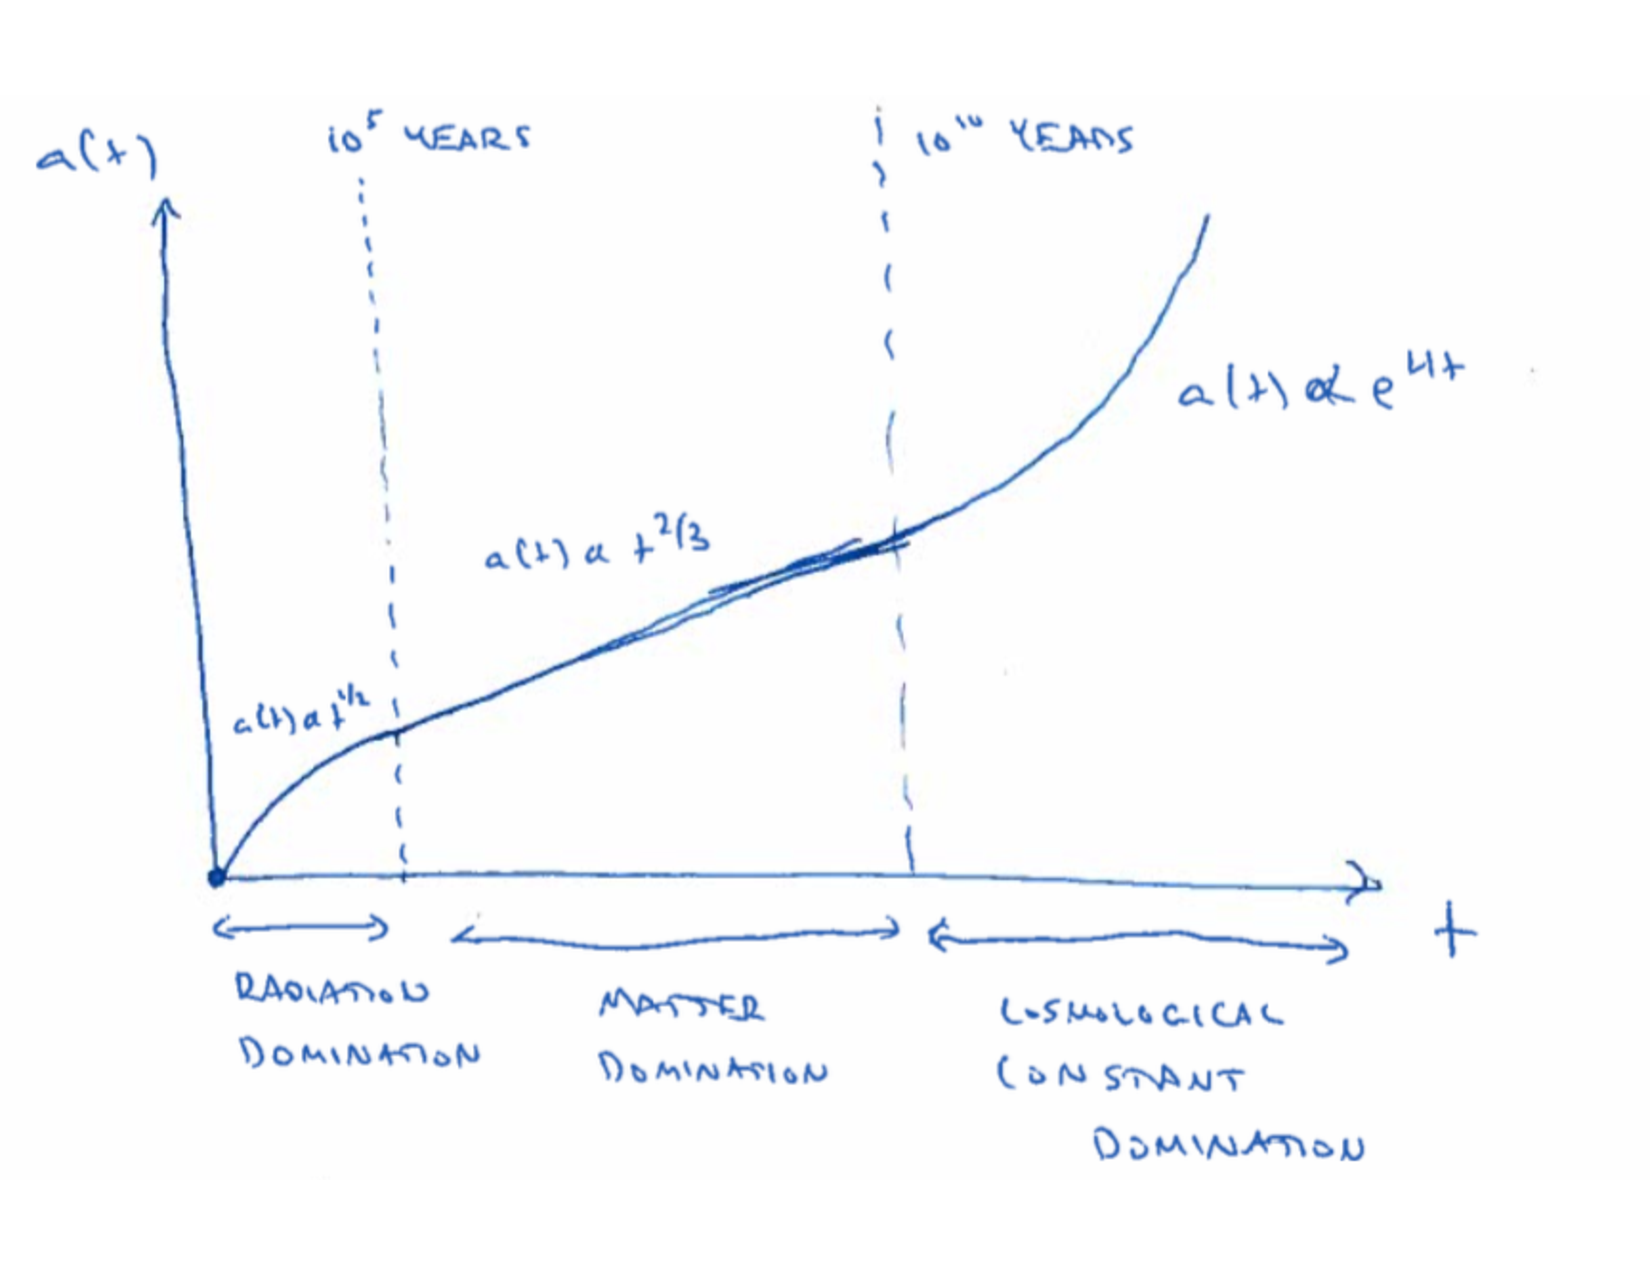
\includegraphics[width=14cm]{figs/lcdm_expansion_history.pdf}}
\caption{Expansion history in $\Lambda$CDM.}
\label{fig:lcdm_expansion_history}
\end{figure}

\item
Given an event in spacetime, we define its {\em comoving coordinates} $(x,y,z)$ to be the spatial
coordinates at $t=t_{\rm today}$ of a comoving observer who passes through the event.  In other words,
the comoving coordinates are the spatial coordinates that would be measured if we wait until today
to make the measurement.

We have now defined global coordinates $(x,y,z,t)$ on spacetime: the comoving spatial coordinates $(x,y,z)$
and the proper time $t$ since the big bang.
We define the {\em comoving distance} $D_c$ between two events $(x,y,z,t)$ and $(x',y',z',t')$ by:
\be
D_c = \sqrt{(x-x')^2 + (y-y')^2 + (z-z')^2}
\ee
In other words, $D_c$ is the distance measured today between two comoving observers who pass through
the events.

\item
If you've taken GR, it may be helpful to say that the expanding universe is described by the
metric $ds^2 = -dt^2 + a(t)^2 (dx^2 + dy^2 + dz^2)$.  The results in this section can all be
derived by doing GR calculations using this metric.  (For example, Eq.~(\ref{eq:photon_redshift}) below
for the photon redshift can be derived by specializing the geodesic equation 
$\ddot x^\mu = \Gamma^\mu_{\nu\rho} \dot x^\nu \dot x^\rho = 0$ to the case
of a null geodesic.)

\item
Now that we have defined global coordinates $(x,y,z,t)$, we can draw spacetime diagrams.
In the left panel of Figure~\ref{fig:frw_lightcone}, we show the past and future lightcones,
using a comoving spatial coordinate $x$ and proper time $t$ on the axes.
(The right panel uses ``conformal time'' as the time coordinate, and will be defined later!)

In this spacetime diagram, lightcones are not at $45^\circ$ angles.  Instead, the lightcone $x(t)$ obeys the
differential equation $dx/dt = a(t)^{-1}$.  This is equivalent to the statement that the physically measured
speed of light is always equal to 1.  Note that $dx/dt$ is the {\em comoving} distance per proper time, so the
physically measured speed (physical distance per proper time) is $a (dx/dt)$.

The size of the past lightcone turns out to be bounded as $a \rightarrow 0$.  That is, the lightcone
comoving coordinate $x(t)$ approaches a finite limit as $t \rightarrow 0$.  (If we assume that $a(t)$
behaves as $a \propto t^{1/2}$ as $t \rightarrow 0$ as shown in Figure~\ref{fig:lcdm_expansion_history},
then this follows since the integral $\Delta x \propto \int a(t)^{-1}$ converges as $t \rightarrow 0$.)
This means that our past causal horizon is finite: there are parts of the universe that have never been
in causal contact with us.  This may be counterintuitive, since you would think that near the big bang
($a=0$) all points in the universe become aribtrarily close to each other, and come into causal contact.

The size of the future lightcone also turns out to be bounded as $a \rightarrow \infty$.
That is, there is a finite patch of the universe that we can ever reach, even if we travel at the speed of light.
(If we assume that $a(t)$ behaves as $a \propto e^{Ht}$ as $t \rightarrow \infty$ as shown in Figure~\ref{fig:lcdm_expansion_history},
then this follows since the integral $\Delta x \propto \int a(t)^{-1}$ converges as $t \rightarrow \infty$.)

\item
In an expanding universe, photons are ``redshifted'': their energy decreases with time.
The physically measured energy $E_{\rm phys}$ measured by a comoving observer scales as:
\be
E_{\rm phys} \propto a(t)^{-1}  \label{eq:photon_redshift}
\ee
(In lecture, I gave a plausibility argument for Eq.~(\ref{eq:photon_redshift}) involving
wavefronts of the electric field, but I didn't reproduce it in the notes!)

\item
We define $\rho(t)$ to be the energy density of the universe at time $t$.
This is a physically measured density, that is, energy per physical (not comoving) volume.
In the standard cosmological model, $\rho(t)$ is the sum of contributions from baryonic matter,
cold dark matter, dark energy, and radiation:
\ba
\rho(t) &=& \mbox{energy density of universe at time $t$} \nn \\
 &=& \rho_b(t) + \rho_c(t) + \rho_\Lambda(t) + \rho_{\rm rad}(t)  \label{eq:lcdm_start}
\ea
Today the densities are:
\ba
\rho(t_{\rm today}) &=& 4.83 \mbox{ keV/cm$^3$}  \\
\rho_b(t_{\rm today}) &=& 0.05 \rho(t_{\rm today})  \\
\rho_c(t_{\rm today}) &=& 0.27 \rho(t_{\rm today})  \\
\rho_\Lambda(t_{\rm today}) &=& 0.68 \rho(t_{\rm today})  \\
\rho_{\rm rad}(t_{\rm today}) &=& (4.15 \times 10^{-5}) \rho(t_{\rm today})
\ea
When talking about expansion history, cosmologists sometimes use the term ``matter''
to mean ``nonrelativistic particles'', and ``radiation'' to mean ``relativistic particles''.
In the standard cosmological model, radiation consists of photons and neutrinos.
(We are assuming for simplicity that the neutrino masses are zero, so that neutrinos are
guaranteed to be relativistic.)
The densities evolve with time as:
\ba
\rho_b(t) &=& a(t)^{-3} \rho_b(t_{\rm today}) \\
\rho_c(t) &=& a(t)^{-3} \rho_c(t_{\rm today}) \\
\rho_\Lambda(t) &=& \rho_\Lambda(t_{\rm today}) \\
\rho_{\rm rad}(t) &=& a(t)^{-4} \rho_{\rm rad}(t_{\rm today})  \label{eq:lcdm_end}
\ea
The time dependence of each component can be understood as follows.
The dark energy is assumed to be a cosmological constant, which by definition
means that $\rho_\Lambda$ is constant in time.
For nonrelativistic particles (baryons and cold dark matter), the energy density
arises from particle rest masses.  As the universe expands,
the number of particles per comoving volume is constant, which implies that the number
density (or energy density $\rho$) per physical volume is proportional to $a^{-3}$.
For relativistic particles (radiation), there is an additional factor $a^{-1}$
since the energy of each particle redshifts with time (Eq.~(\ref{eq:photon_redshift})),
leading to an overall time dependence of the form $\rho_{\rm rad} \propto a^{-4}$.

Taken together, Eqs.~(\ref{eq:lcdm_start})--(\ref{eq:lcdm_end}) specify the energy
density of each component $\rho_i$, and the total energy density $\rho$, as a 
function of the scale factor $a$.  At very early times (roughly $a \lesssim 1/3000$),
radiation is the dominant component of the universe, since its energy density scales
as $a^{-4}$.  Next, the universe is matter dominated until $a \sim 0.7$, when it starts
to become cosmological constant dominated.

\item
So far, we have not explained how the time dependence of $a(t)$ shown in Figure~\ref{fig:lcdm_expansion_history} arises.
The evolution of $a(t)$ is determined by {\em Friedmann's equation}, which relates the expansion rate to the energy density:
\be
\left( \frac{1}{a} \frac{da}{dt} \right)^2 = \frac{8\pi G}{3} \rho(t)
\ee
As a bit of notation, the {\em Hubble expansion rate} $H(t)$ is defined to be the fractional expansion rate per unit time:
\be
H(t) = \frac{1}{a} \frac{da}{dt}
\ee
and another way of writing Friedmann's equation is:
\be
H^2 = \frac{8\pi G}{3} \rho
\ee

\item
The ``plot'' of $a(t)$ in Figure~\ref{fig:lcdm_expansion_history} can be obtained by integrating
Friedmann's equation as follows.  First, we write $\rho(a)$ as follows.
\be
\rho(a) = \rho_0 \left( \Omega_\Lambda + \Omega_b a^{-3} + \Omega_c a^{-3} + \Omega_{\rm rad} a^{-4} \right)
\ee
where we have introduced some standard cosmology notation: $\rho_0 = \rho(t_{\rm today})$ is the
energy density today, and $\Omega_i = \rho_i(t_{\rm today}) / \rho(t_{\rm today})$ is the fractional
density of component $i$ today (where $i \in \{ b, c, \Lambda, {\rm rad} \}$).

Second, we use Friedmann's equation to write $H(a)$ as
\be
H(a) = H_0 \left( \Omega_b a^{-3} + \Omega_c a^{-3} + \Omega_\Lambda + \Omega_{\rm rad} a^{-4} \right)^{1/2}
\ee
where $H_0 = (8\pi G \rho_0 / 3)^{1/2}$ is the Hubble expansion rate today.

Third, we integrate to get $t$ as a function of $a$.
\ba
\frac{dt}{da} &=& \frac{1}{a H(a)} \\
t &=& \int_0^a \frac{da'}{a' \, H(a')} \nn \\
 &=& H_0^{-1} \int_0^a da' \, (a')^{-1} \left( \Omega_b a^{-3} + \Omega_c a^{-3} + \Omega_\Lambda + \Omega_{\rm rad} a^{-4} \right)^{-1/2}
\ea
This integral cannot be done analytically, but it is straightforward to integrate numerically.
For example, if we integrate from $a=0$ to $a=1$, we get the age of the universe, which turns out to be $t=1.38 \times 10^{10}$ years.

\item
Let's look at an example where Friedmann's equation can be integrated analytically.
Suppose the density $\rho$ is a power law in the scale factor $a$:
\be
\rho(a) = \rho_0 a^{-3(1+w)}  \label{eq:constant_w}
\ee
We have written the exponent as $3(1+w)$ to conform to some standard notation in cosmology.
The parameter $w$ defined in Eq.~(\ref{eq:constant_w}) can be interpreted as the ratio $w = p/\rho$,
where $p$ is the total pressure of the universe, and $w$ is called the ``equation of state''.

The power-law cosmology we are considering is called a ``constant-$w$ cosmology''.
It includes the following special cases:
\begin{itemize}
\item A ``matter dominated'' universe, where the energy density is dominated by nonrelativistic particles ($w=0$).
\item A ``radiation dominated'' universe, where the energy density is dominated by relativistic particles ($w=1/3$).
\item A cosmological constant dominated universe ($w=-1$).
\end{itemize}
Note that the $\Lambda$CDM universe is radiation dominated at early times, and cosmological
constant dominated at late times.

\item
In the constant-$w$ universe defined by Eq.~(\ref{eq:constant_w}), Friedmann's equation can be integrated as follows:
\ba
H(a) 
  &=& \left( \frac{8\pi G}{3} \rho(a) \right)^{1/2} \nn \\
  &=& H_0 a^{-3(1+w)/2} \hspace{2cm} \mbox{where } H_0 = \left( \frac{8\pi G}{3} \rho_0 \right)^{1/2} \\
\frac{dt}{da} 
  &=& \frac{1}{aH} \\
t
  &=& \int \frac{da}{a H(a)} \nn \\
  &=& H_0^{-1} \int da \, a^{(1+3w)/2}  \label{eq:constw_t}
\ea
Depending on the value of $w$, this integral may or may not converge, in the limits $a\rightarrow 0$ and $a \rightarrow \infty$.
\ba
\mbox{(Integral in Eq.~(\ref{eq:constw_t}) converges as $a\rightarrow 0$)}
 & \Leftrightarrow &
\mbox{(Universe begins in a big bang)} \nn \\
 & \Leftrightarrow &
w > -1 \\
\mbox{(Integral in Eq.~(\ref{eq:constw_t}) converges as $a\rightarrow \infty$)}
 & \Leftrightarrow &
\mbox{(Universe ends in a ``big rip'')} \nn \\
 & \Leftrightarrow &
w < -1
\ea
For $\Lambda$CDM, we have $w=1/3$ at early times and $w=-1$ at late times,
so the universe begins in a big bang singularity, but does not end in a big
rip singularity (barely!)

\item
Continuing to assume the constant-$w$ universe defined by Eq.~(\ref{eq:constant_w}), let's
solve for the trajectory $x(t)$ of a light ray.  Here, $x$ is a comoving spatial coordinate
and $t$ is proper time.  Previously, we argued that the trajectory was determined by the
differential equation $dx/dt = 1/a(t)$.  Therefore,
\ba
x &=& \int \frac{dt}{a} \nn \\
  &=& \int \frac{da}{a^2 H(a)} \nn \\
  &=& H_0^{-1} \int da \, a^{(-1+3w)/2}  \label{eq:constw_x}
\ea
Depending on the value of $w$, this integral may or may not converge, in the limits $a\rightarrow 0$ and $a \rightarrow \infty$.
\ba
\mbox{(Integral in Eq.~(\ref{eq:constw_x}) converges as $a\rightarrow 0$)}
 & \Leftrightarrow &
\mbox{(Past causal horizon is finite)} \nn \\
 & \Leftrightarrow &
w > -\frac{1}{3} \\
\mbox{(Integral in Eq.~(\ref{eq:constw_x}) converges as $a\rightarrow \infty$)}
 & \Leftrightarrow &
\mbox{(Future causal horizon is finite)} \nn \\
 & \Leftrightarrow &
w < -\frac{1}{3}
\ea
For $\Lambda$CDM, we have $w=1/3$ at early times and $w=-1$ at late times,
so the past and future causal horizons are both finite (as previously stated).

\item
As you can see from the calculations in the last few bullet points, 
it is useful to switch between time coordinates $t$ and $a$.
There are a few more time coordinates which are useful in cosmology.
First, the redshift $z$, which is related to $a$ by the change of variables:
\be
a = \frac{1}{1+z}
\ee
By convention, physicists usually use $a$, whereas astronomers use $z$,
but there is no real difference.

\item
Another useful time coordinate is {\em conformal time} $\tau$, which is defined by
the differential equation
\be
\frac{d\tau}{dt} = \frac{1}{a(t)}
\ee
with initial condition $\tau=0$ at the big bang ($a=0$).  Some equivalent definitions:
\ba
\tau
  &=& \int_0^t \frac{dt'}{a(t')} \nn \\
  &=& \int_0^a \frac{da'}{a'{}^2 \, H(a')}
\ea
This time coordinate has the property that ``lightcones are at $45^\circ$ angles'',
that is, the trajectory of a light ray is $dx/d\tau=1$.

\item
 There are multiple notions of time and distance in an expanding universe.
 For example, the age of the universe $(\Delta t)$ is 14 billion years old, 
 but the size of the observable universe $(\Delta x$) is 46 billion comoving light-years.
 That is, if we look back to the big bang along our past lightcone, the resulting point in space
 would be 46 billion light-years away today.  (Figure~\ref{fig:frw_lightcone}, left panel.)

 Because lightcones are $45^\circ$ in conformal time, the conformal age of the universe ($\Delta\tau$)
 is the same as the size of the observable universe $(\Delta x)$, i.e.~46 billion comoving light-years.
 (Figure~\ref{fig:frw_lightcone}, right panel.)  In general, you can think of conformal time as ``comoving distance
 along the lightcone''.

\begin{figure}[h!]
\centerline{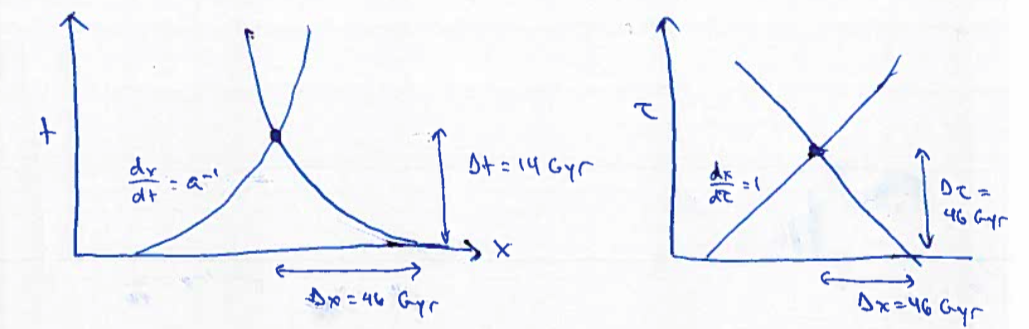
\includegraphics[width=14cm]{figs/frw_lightcone.png}}
\caption{FRW lightcone geometry in proper time $t$ (left) and conformal time $\tau$ (right),
  and comoving spatial coordinate $x$.}
\label{fig:frw_lightcone}
\end{figure}

\end{itemize}

\par\noindent
This concludes our main discussion of the expanding universe.
In the following bullet points, we mention a few additional points for completeness,
in less detail (we just sketch the key equations).
These points will either not be used at all in the next section, or will only be used
briefly.

\begin{itemize}

\item
So far we have analyzed the dynamics of massless particles (photons), 
which are fully described by the statements that the trajectory satisfies $dx/dt=a(t)^{-1}$, 
and the photon energy redshifts as $E \propto a^{-1}$.  
Let us now consider the case of massive particles.
We will state the main results without derivation, since the derivation requires GR.
These results will be used briefly at the end of the next section, in the context of massive neutrinos.

A massive particle has a 4-momentum ($E_{\rm phys}$, $p_{\rm phys}$), where
\be
E_{\rm phys} = \frac{m_0}{\sqrt{1-v^2}}
  \hspace{1cm}
p_{\rm phys} = \frac{m_0 v}{\sqrt{1-v^2}}
\ee
If the particle is moving in the expanding universe with no applied force,
then the momentum redshifts as $p_{\rm phys} \propto a^{-1}$.  This statement
is true for both massive and massless particles, and generalizes our previous
statement that photon energies redshift as $a^{-1}$.  Note that for a massive
particle, the velocity eventually $v$ becomes arbitrarily small as the universe
expands.

If an external force $F$ acts on a massive particle, then
\be
\frac{dp_{\rm phys}}{dt} = - H p_{\rm phys} + F
\ee
The term $(-H p_{\rm phys})$ is a gravitational force (sometimes called ``Hubble friction'' or ``Hubble drag'')
which slows down particles in the cosmic rest frame.

\item
A few more definitions.
Let $p(t)$ be the total pressure of the universe, defined as follows.

Operational definition: consider an ensemble of particles with physical number density $n_{\rm phys}$
and 4-momentum $(E_{\rm phys}, p_{\rm phys})$.  (We assume that the magnitude of each particle's momentum
is the same, but the directions of the momenta are uniformly distributed.)  Then:
\be
\rho(t) = n_{\rm phys} E_{\rm phys}
  \hspace{1cm}
p(t) = n_{\rm phys} \left( \frac{p_{\rm phys}^2}{3 E_{\rm phys}} \right)  \label{eq:p_operational}
\ee
Note that we have $p(t) \rightarrow 0$ and $p(t) \rightarrow \rho(t)/3$ in the nonrelativistic
and relativistic limits respectively.

Conceptual definition: suppose we place a 3D ``box'' anywhere in the universe, and assume
that particles bounce elastically from the sides the box.  Then $p(t)$ is the force per
unit area on the sides of the box.

Here are two important equations, which we haven't mentioned so far:
\begin{align}
\frac{d\rho}{d\log a} &= -3(\rho + p)  & \mbox{(``Continuity equation'')} \\
\frac{dH}{dt} &= -4\pi G (\rho + p) & \mbox{(``Friedmann's second equation'')}
\end{align}
The continuity equation generalizes the law of conservation of energy to the expanding
universe, and can be integrated to give the evolution of the energy density $\rho$.
We haven't needed the continuity equation yet, because we have been considering
particle species in either the nonrelativistic or relativistic limits, where we argued directly
that the energy density evolves as $a^{-3}$ or $a^{-4}$ respectively.  However, in an
intermediate case (say $v=0.5c$), we would need the continuity equation.

Friedmann's second equation is equivalent to the continuity equation (if Friedmann's
first equation is assumed), but is sometimes convenient on its own.

\item
So far, we have assumed that the universe is spatially flat.
There is a generalization where the universe is allowed to have spatial curvature,
which we now sketch.  (These results won't be used in the rest of the notes, and
weren't included in the lecture, except in response to a question!)

First, we consider the case of positive curvature, that is a sphere of
comoving radius $R_c$.  (The comoving radius is fixed throughout the
expansion.)  Then Friedmann's equation becomes:
\be
H^2 + \frac{K}{a^2} = \frac{8\pi G}{3} \rho
  \hspace{1cm}
\mbox{where $K = 1/R_c^2$}
\ee
(Derivation omitted, since it requires GR!)

The effect of positive curvature is the same as a {\em negative}
contribution to the energy density, of the form
\be
\rho_K = - \frac{3}{8\pi G} \frac{K}{a^2} \label{eq:rho_K}
\ee
Through analysis of the CMB and other datasets, curvature is known to be small.
The current observational bound is roughly:
\be
|\Omega_K| = \left| \frac{\rho_K(a=1)}{\rho_{\rm tot}(a=1)} \right| \lsim 10^{-2}
\ee
Since $\rho_K \propto a^{-2}$, it follows that curvature is also small at all times
in the expansion history, since at early times it is dominated by matter ($a^{-3}$)
or radiation ($a^{-4}$), and at late times it is dominated by the cosmological constant.

The curvature $K$ can also be negative.  In this case, the spatial geometry is a
hyperboloid rather than a sphere.  The corresponding contribution to the energy
density (Eq.~(\ref{eq:rho_K})) is positive.

\end{itemize}

\section{Thermal history}

\begin{itemize}

\item
Today, the cosmic microwave background is a blackbody with temperature $T = 2.726$ Kelvin.
As the universe expands, the temperature decreases as $T \propto a^{-1}$.  (This is not obvious,
but starting from the standard formula for the blackbody spectrum, one can show that if every
photon redshifts as $1/a$, the result is another blackbody spectrum with temperature $T/a$.)

Therefore, if we imagine looking back to the early universe, the universe will get hotter and 
denser at earlier times.  At a time when the temperature is $\approx 3000$ K, corresponding to
scale factor $a = 10^{-3}$, something interesting happens.  Above this temperature, there are
enough high-energy CMB photons to ionize neutral hydrogen atoms into free protons and electrons.
Therefore, as the universe expands and cools, it transitions from an opaque $p^+e^-$ plasma to a gas
of transparent neutral hydrogen.  This is the time when the CMB is formed.

\item
Continuing to go back in time, another interesting event in the thermal history occurs at $T = 0.5$ MeV,
when the temperature is equal to the electron mass.  Above this temperature, there are enough high-energy
photons to produce $e^+e^-$ pairs via the process $2\gamma \rightarrow e^+e^-$, and the universe is a
plasma of photons, positrons and electrons (plus a few protons and neutrons).  Below this temperature,
the positrons and electrons have mostly annihilated to photons, and their abundance is small.  

(As an aside, you might wonder why there are still electrons in the universe today.  This is because there is
a small asymmetry between the abundance of positrons and electrons in the initial conditions, so that some electrons
remain after all the positrons have annihilated.  The reason for this initial asymmetry is still an unsolved problem
in cosmology!)

\item
Going slightly further back in the thermal history, another interesting event occurs at $T = 1$ MeV.
Above this temperature, neutrinos are in thermal equilibrium with the $e^+e^-\gamma$ plasma, due to
scattering processes like $\nu e^- \rightarrow \nu e^-$ or $e^+e^- \rightarrow \nu \bar \nu$.
Below this temperature, these scattering events become infrequent enough that the neutrinos decouple
from the thermal plasma and can be treated as noninteracting.  This event is called ``neutrino freezeout''.

\item
The preceding events in the thermal history are shown in Figure~\ref{fig:thermal_history}.
Note that there are many interesting events not shown!
For example, at 100 keV, the electroweak interactions which convert protons to neutrons freeze out,
and the cosmological abundance of neutrons (and other atomic nuclei, such as lithium) is determined.
This stage in the thermal history is called ``Big Bang Nucleosynethesis'', but we won't cover it in these notes.
Our goal in this section is to analyze the ``neutrino freezeout'' and ``$e^+e^-$ annihilation'' stages,
and show how they {\em predict a cosmic neutrino background with temperature} $T_\nu = (4/11)^{1/3} T_{\rm CMB} = 1.95$ Kelvin.

% Note: Syntax for clipping a figure is
% \includegraphics[trim={5cm 0 0 0},clip,...]
%  where ordering is <left> <lower> <right> <upper>
\begin{figure}[h!]
\centerline{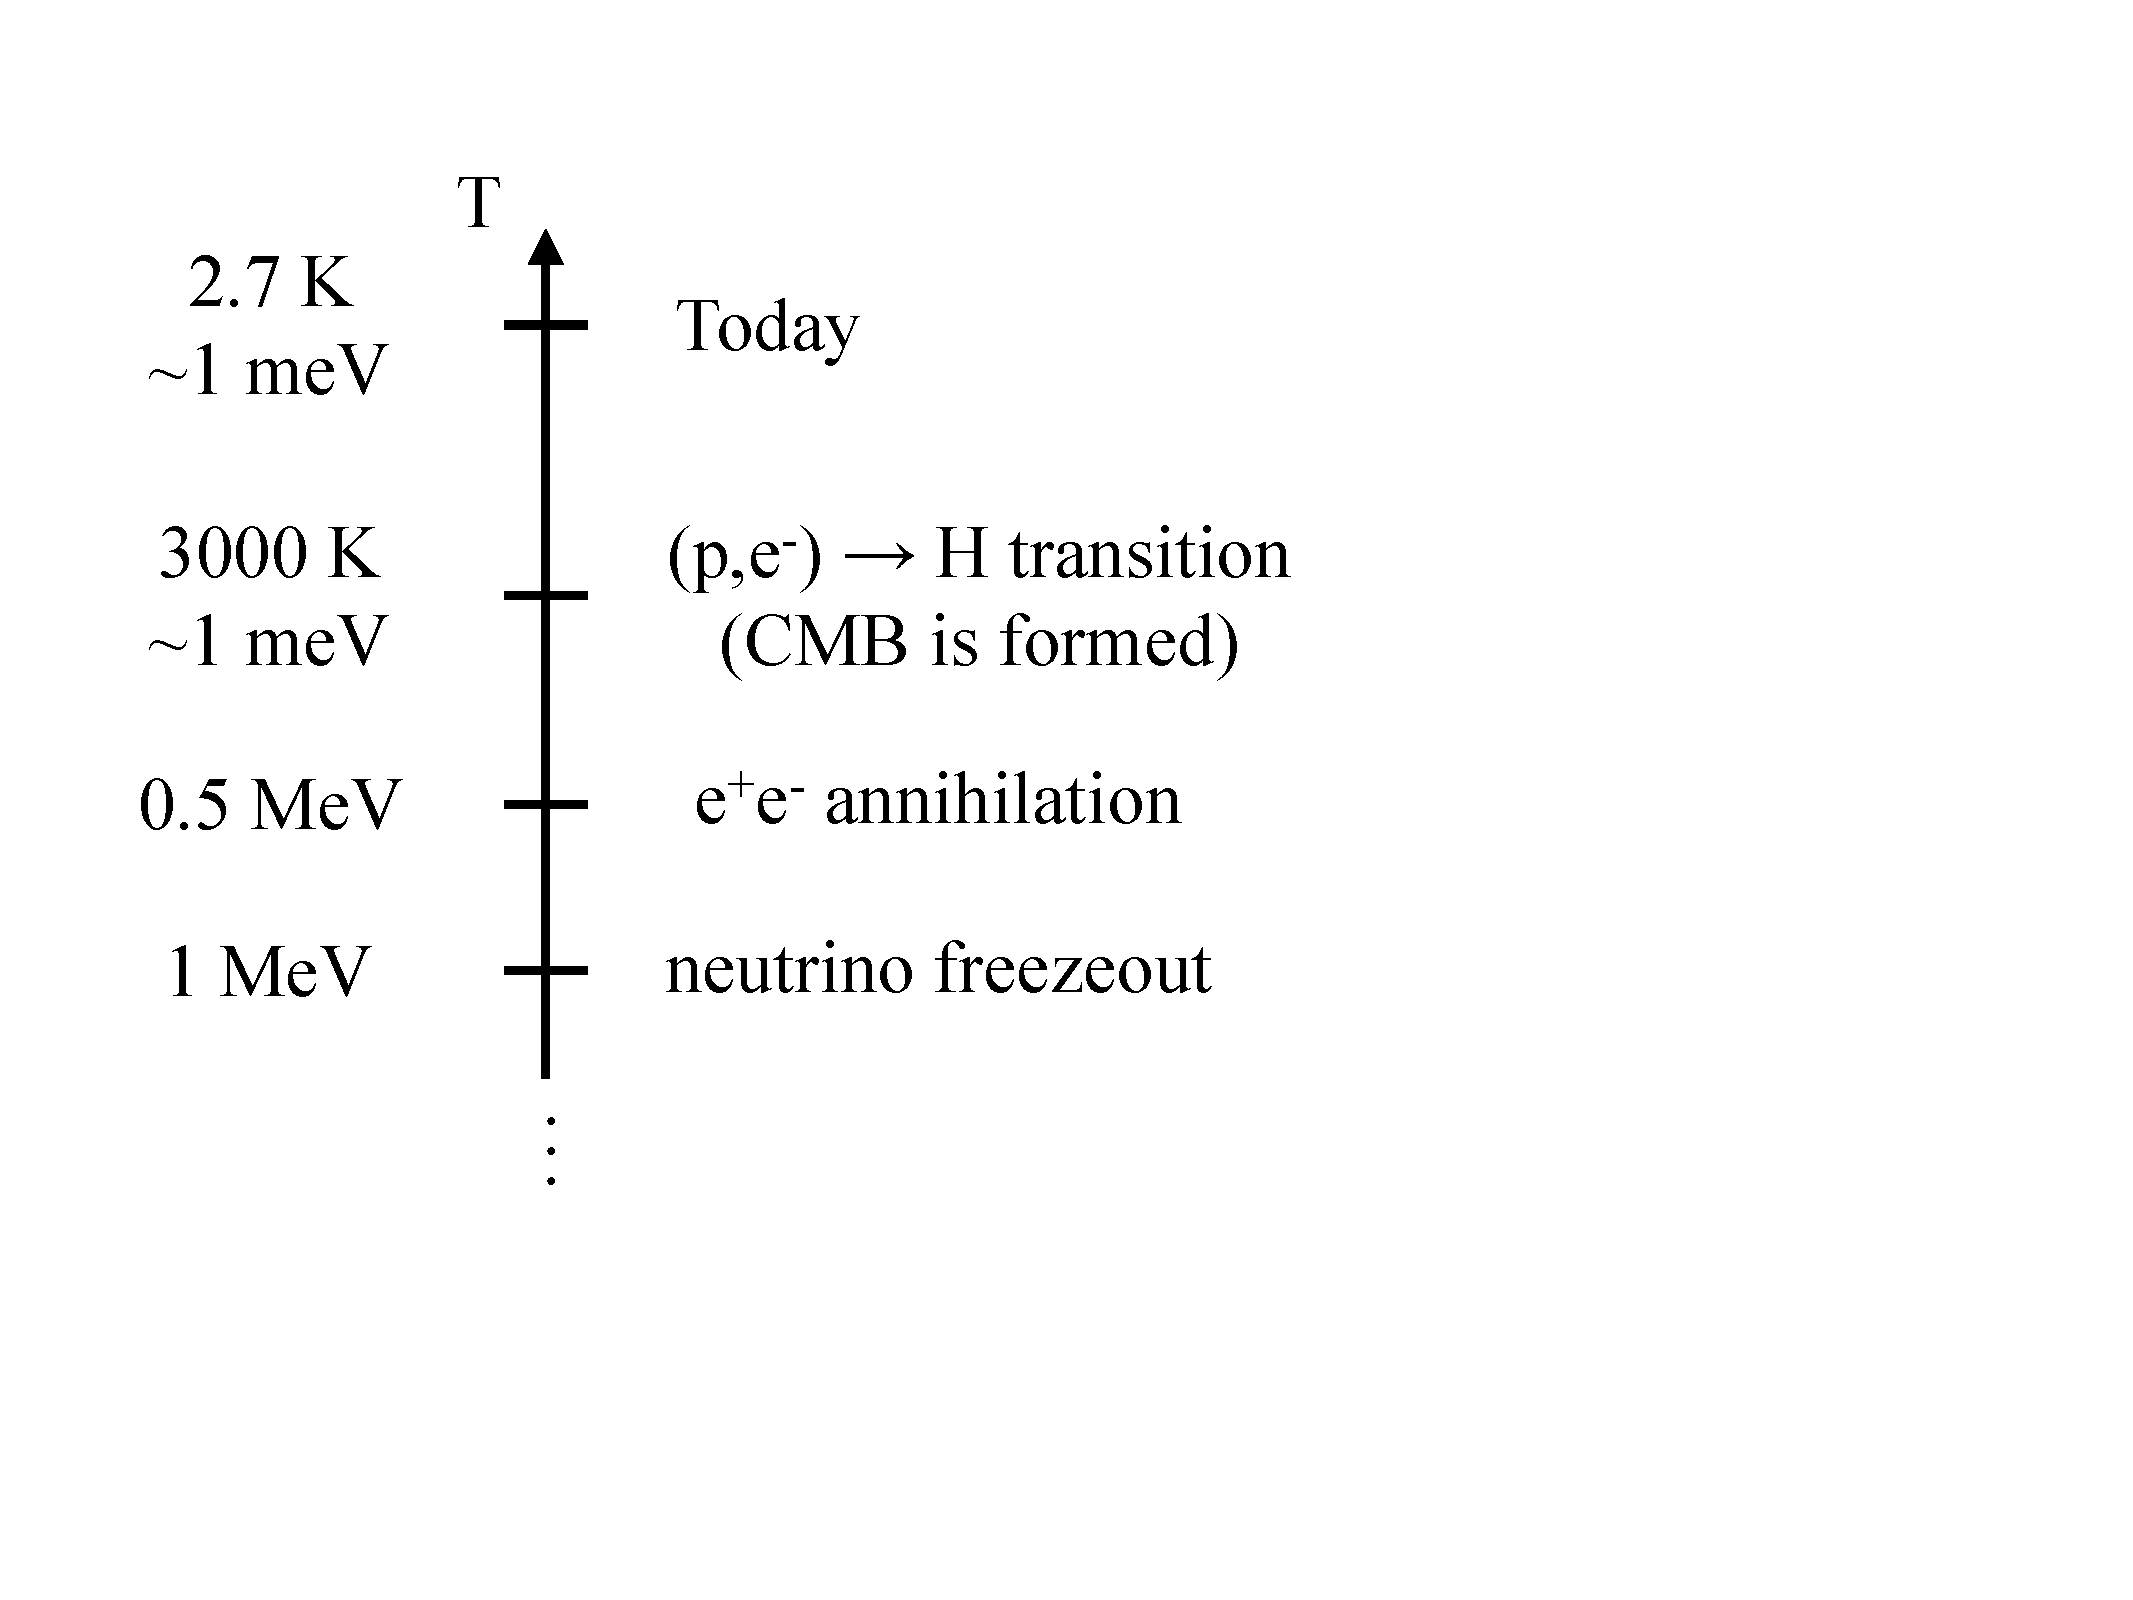
\includegraphics[trim={0 6cm 12cm 2cm},clip,width=6cm]{figs/thermal_history.pdf}}
\caption{Thermal history of the universe.  (With some interesting steps omitted, for example Big Bang Nucleosynthesis at $T=100$ keV!)}
\label{fig:thermal_history}
\end{figure}

\item
As a starting point for analyzing the thermal history,
consider a box of volume $V$, containing a multiparticle plasma at temperature $T$.
The plasma can consist of multiple particle species.
Each species can be a boson or fermion, massive or massless, and can have arbitrary spin.
We will assume that all multiparticle states are in thermal equilibrium, so that the probability
of every multiparticle state is given by the Boltzmann distribution $\propto e^{-E/T}$, where
$E$ is the total energy of the state (obtained by summming the energies of all particles).

\item 
Consider a single momentum $p$, a single particle species with rest mass $m$, and a single spin state.
This defines a mode, whose occupation number $N$ will be a random number whose probability distribution
is given by the Boltzmann distribution:
\be
p(N) \propto e^{-NE_p/T}
  \hspace{1cm}
\mbox{where $E_p = \sqrt{p^2+m^2}$}
\ee
We will be interested in calculating the expectation value $f_p = \langle N \rangle$.
If the particle is a fermion, then $N$ can be either $0$ or $1$, and:
\begin{align}
p(N) &= \frac{e^{-NE_p/T}}{1 + e^{-E_p/T}}  & \mbox{(fermion assumed)}  \\
f_p &= \sum_{N=0}^1 N p(N) \nn \\
   &= \frac{e^{-E_p/T}}{1 + e^{-E_p/T}} & \mbox{(fermion assumed)}  \label{eq:fp_fermion}
\end{align}
If the particle is a boson, then $N$ can be any integer, and:
\begin{align}
p(N) &= \frac{e^{-NE_p/T}}{\sum_{N=0}^\infty e^{-NE_p/T}} & \mbox{(boson assumed)} \\
f_p &= \sum_{N=0}^\infty N p(N) \nn \\
 &= \frac{\sum_{N=0}^\infty N e^{-NE_p/T}}{\sum_{N=0}^\infty e^{-NE_p/T}} \nn \\
 &= \frac{e^{-E_p/T} (1 - e^{-E_p/T})^{-2}}{(1 - e^{-E_p/T})} \nn \\
 &= \frac{e^{-E_p/T}}{1 - e^{-E_p/T}} & \mbox{(boson assumed)}  \label{eq:fp_boson}
\end{align}
where we have used Eqs.~(\ref{eq:geom_series}),~(\ref{eq:geom_series2}).
We see that Eqs.~(\ref{eq:fp_fermion}),~(\ref{eq:fp_boson}) may be combined into the single expression:
\be
f_p = \frac{e^{-E_p/T}}{1 \mp e^{-E_p/T}} \label{eq:fp}
\ee
where {\em in Eq.~(\ref{eq:fp}) and throughout this section, the upper sign means ``boson'', and the lower sign means ``fermion''}.

\item
Now we would like to compute the total energy density, by summing over all momenta, spin states, and particle species.
When we sum over momenta in a box with volume $V$, we will replace the sum by the following ``mode-counting'' integral:
\be
\sum_p \rightarrow V \int \frac{d^3p}{(2\pi)^3}  \label{eq:mode_counting}
\ee
To derive this, suppose that the side lengths of the box are $(L_x, L_y, L_z)$, with $V = L_x L_y L_z$,
and the box has periodic boundary conditions.
In such a box, the momentum $p = (p_x, p_y, p_z)$ of a particle must be quantized as:
\be
(p_x, p_y, p_z) = \left( \frac{2\pi}{L_x} n_x, \frac{2\pi}{L_y} n_y, \frac{2\pi}{L_z} n_z \right)  
  \hspace{1cm} \mbox{($(n_x,n_y,n_z)$ integers)} \label{eq:p_quantization}
\ee
in order for the wavefunction $\psi(x) = e^{ip\cdot x}$ to satisfy the periodic boundary conditions.
Therefore, when we sum over momenta, we are summing over a discrete lattice of momenta defined by Eq.~(\ref{eq:p_quantization}).
A little thought shows that the number of lattice elements per volume $(d^3p)$ is $(L_xL_yL_z)/(2\pi)^3 = V/(2\pi)^3$.
Therefore, the sum over momenta can be approximated by the integral $\int d^3p \, V / (2\pi)^3$.
This completes the derivation of Eq.~(\ref{eq:mode_counting}).

\item
Now we can compute the energy density of the plasma:
\ba
\rho 
  &=& \frac{1}{V} \sum_{\rm species} \sum_{\rm spins} \sum_p E_p f_p \nn \\
  &=& \frac{1}{V} \sum_{\rm species} g V \int \frac{d^3 p}{(2\pi)^3} E_p \frac{e^{-E_p/T}}{1 \mp e^{-E_p/T}} \nn \\
  &=& \sum_{\rm species} \frac{g}{2\pi^2} \int dp \, p^2 E_p \frac{e^{-E_p/T}}{1 \mp e^{-E_p/T}}  \label{eq:rho_exact1}
\ea
Here, $g$ denotes the number of spin states (which can be different for each particle species).
The integral in Eq.~(\ref{eq:rho_exact1}) gives the exact energy density $\rho$, for a particle with
arbitrary mass and spin.  For arbitrary $m$ the integral cannot be done analytically, but we will
be able to determine the leading behavior in the relativistic limit $T \gg m$ and nonrelativistic
limit $T \ll m$, in the next two bullet points.

\item
First consider the relativistic limit ($T \gg m$).  In this case we can approximate $E_p \approx p$ in the integral:
\ba
\rho 
  &=& \frac{g}{2\pi^2} \int dp \, p^2 E_p \frac{e^{-E_p/T}}{1 \mp e^{-E_p/T}} \nn \\
  & \approx & \frac{g}{2\pi^2} \int dp \, p^3 \frac{e^{-p/T}}{1 \mp e^{-p/T}} \nn \\
  & = & \frac{g}{2\pi^2} \int dp \, p^3 \left( e^{-p/T} \pm e^{-2p/T} + e^{-3p/T} \pm e^{-4p/T} + \cdots \right) \nn \\ 
  & = & \frac{g}{2\pi^3} (6 T^4) \times \left\{ \begin{array}{cl} 
     (\pi^4/90) & \mbox{[boson]} \\
     (7/8) (\pi^4/90) & \mbox{[fermion]}
  \end{array} \right.
\ea
In the last line we have used Eqs.~(\ref{eq:gamma}),~(\ref{eq:zeta4}), and~(\ref{eq:zeta4a}).
In the cosmology literature, the result is usually written this way:
\be
\rho \approx \frac{\pi^2}{30} g_* T^4 \hspace{1cm} (\mbox{$T \gg m$ assumed})
\ee
where we have defined
\be
g_* = \left\{ \begin{array}{cl}
  g & \mbox{[boson]} \\
 (7/8) g & \mbox{[fermion]}
\end{array} \right.
\ee
This result generalizes the usual expression $\rho = (\pi^2/15) T^4$ for the energy
density of blackbody radiation (for photons, $g=g_*=2$).

\item
Now consider the nonrelativistic limit ($T \ll m$).  In this case:
\begin{align}
\rho 
  & = \frac{g}{2\pi^2} \int dp \, p^2 E_p \frac{e^{-E_p/T}}{1 \mp e^{-E_p/T}} \nn \\
  & \approx \frac{g}{2\pi^2} \int dp \, p^2 E_p e^{-E_p/T} \nn \\
  & = \frac{g}{2\pi^2} \int_m^\infty dE \, E^2 \sqrt{E^2-m^2} e^{-E/T}  
    & \mbox{change variable $E = \sqrt{p^2+m^2}$} \nn \\
  & = \frac{g}{2\pi^2} e^{-m/T} \int_0^\infty d\epsilon \, (m+\epsilon)^2 \epsilon^{1/2} (2m+\epsilon)^{1/2} e^{-\epsilon/T}
    & \mbox{change variable $\epsilon = E-m$} \nn \\
  & \approx \frac{g}{2\pi^2} e^{-m/T} \int_0^\infty d\epsilon \, m^2 \epsilon^{1/2} (2m)^{1/2} e^{-\epsilon/T} \nn \\
  & = \frac{g}{2\pi^2} e^{-m/T} m^2 (2m)^{1/2} \frac{\sqrt{\pi}}{2} T^{3/2} \nn \\
  & = gm \left( \frac{mT}{2\pi} \right)^{3/2} e^{-m/T}
\end{align}
where we have used Eq.~(\ref{eq:gamma}) to do the integral (note that $(1/2)! = \sqrt{\pi}/2$).
We see that the abundance of a massive particle is exponentially suppressed when the temperature
of the plasma falls below the particle mass.

\item
Summarizing the previous bullet points, for a single particle species, the energy
density $\rho$ is given by:
\ba
\rho(T) &=& \frac{g}{2\pi^2} \int dp \, p^2 E_p \frac{e^{-E_p/T}}{1 \mp e^{-E_p/T}}  \label{eq:rho_exact2} \\
  &=& \left\{ \begin{array}{cl}
   \frac{\pi^2}{30} g_* T^4 & (T \gg m) \\
   gm \left( \frac{mT}{2\pi} \right)^{3/2} e^{-m/T} & (T \ll m)  \label{eq:rho_limits}
\end{array} \right.
\ea

\item
We will also need formulas for the pressure $p$, which was defined briefly near the previous section.
According to Eq.~(\ref{eq:p_operational}), a particle with 4-momentum $(E,p)$ contributes $E$ to the
total energy and $(p^2/3E)$ to the pressure.  Therefore, the pressure is given by the following integral,
which was obtained by replacing $E_p$ in Eq.~(\ref{eq:rho_exact2}) by $p^2/(3E_p)$:
\be
p(T) = \frac{g}{2\pi^2} \int dp \, p^2 \left( \frac{p^2}{3E_p} \right) \frac{e^{-E_p/T}}{1 \mp e^{-E_p/T}}  \label{eq:p_exact}
\ee
As in the case of the density $\rho$, the leading behavior of this integral in the relativistic
and nonrelativistic limits can be calculated analytically.  We omit the details and quote the final result:
\be
p(T)
  = \left\{ \begin{array}{cl}
   (1/3) \rho(T) & (T \gg m) \\
   (T/m) \rho(T) & (T \ll m)
\end{array} \right.  \label{eq:p_limits}
\ee

\item
So far, we have not considered the expansion of the universe.
We would like to know how the temperature $T$ of the plasma evolves with the scale factor $a$.
In principle, this can be determined by using the continuity equation, which was mentioned near the end of the last section:
\be
\frac{d\rho}{d\log a} = -3(\rho + p) \label{eq:continuity2}
\ee
Since $\rho$ and $p$ are functions of $T$, given explicitly by Eqs.~(\ref{eq:rho_exact2}),~(\ref{eq:p_exact}) above,
the continuity equation (a single first-order differential equation) suffices to determine $T(a)$ (since there is
only one dynamical degree of freedom, the temperature $T$).

For example, if we assume $p = \rho/3$, which is a good approximation if all species are relativistic (Eq.~(\ref{eq:p_limits})), then
the continuity equation reads $d\rho/d\log a = -4\rho$, which implies $\rho \propto a^{-4}$.  If all species
are relativistic, then we also know that $\rho \propto T^4$ (Eq.~(\ref{eq:rho_limits})), so this implies
$T \propto a^{-1}$.

Note that most of the time, all species in the plasma are relativistic, and $T$ evolves as $T \propto a^{-1}$.
This is because when a species becomes nonrelativistic, its abundance becomes exponentially suppressed, and it can be neglected.
For example, if the temperature is significantly higher than 0.5 MeV (say 2 MeV), then the plasma consists of positrons, electrons,
and photons, and all species are relativistic.
If the temperature is significantly lower than 0.5 MeV (say 0.1 MeV), then the plasma consists only of photons (which are always
relativistic), and the $e^+e^-$ abundance is small enough to be negligible.
In both of these regimes, the temperature evolves as $T \propto a^{-1}$.
During the $e^+e^-$ annihilation event when $T \sim 0.5$ MeV, the evolution of the temperature is more complicated,
but in principle it can be obtained from the continuity equation (Eq.~(\ref{eq:continuity2})).

\item
In fact, the continuity equation can be integrated exactly, to give the evolution of $T$ for all values of the
scale factor $a$, including the behavior during annihilation events.  The exact solution can be written as the
following conservation law:
\be
a^3 \left( \frac{\rho(T) + p(T)}{T} \right) = \mbox{const.}  \label{eq:s_const}
\ee
This conservation law is nontrivial to derive, and there is more than one way of deriving it.
In the next two bullet points, we will use a brute-force approach based on the continuity approach.
This has the advantage of being completely rigorous, but the disadvantage that the conservation law
in Eq.~(\ref{eq:s_const}) looks like an algebraic accident.

There is also a thermodynamic derivation based on identifying the quantity $(\rho+p)/T$ as the entropy
per unit physcal volume, and arguing that the expansion of the universe should be an adiabatic process
which conserves entropy per comoving volume.  In these notes, we omit the thermodynamic derivation!

\item
As a first step toward proving the conservation law in Eq.~(\ref{eq:s_const}), we prove the following lemma:
\be
\frac{\partial p}{\partial T} = \frac{\rho + p}{T}  \label{eq:lemma_dpdT}
\ee
The proof is as follows.  First, we take the integral expressions for $\rho$ and $p$ in Eqs.~(\ref{eq:rho_exact2}),~(\ref{eq:p_exact}),
and change variables to $E = \sqrt{p^2+m^2}$, obtaining:
\ba
\rho &=& \frac{g}{2\pi^2} \int dE \, E^2 \sqrt{E^2-m^2} f(E/T)  \label{eq:rho_Eintegral} \\
p &=& \frac{g}{2\pi^2} \int dE \, \left( \frac{1}{3} (E^2-m^2)^{3/2} \right) f(E/T)  \label{eq:p_Eintegral}
\ea
where $f(E/T) = e^{-E/T} / (1 \mp e^{-E/T})$.
In this equation and others below, integrals over $E$ run from $E=m$ to $E=\infty$.
Now, starting from Eq.~(\ref{eq:p_Eintegral}), we calculate $(\partial p/\partial T)$ as follows:
\ba
\frac{\partial p}{\partial T}
 &=& \frac{g}{2\pi^2} \int dE \, \left( \frac{1}{3} (E^2-m^2)^{3/2} \right) \left( - \frac{E}{T^2} \right) f'(E/T) \nn \\
 &=& \frac{g}{2\pi^2} \int dE \, \left( \frac{1}{3} (E^2-m^2)^{3/2} \right) \left( - \frac{E}{T} \right) \frac{\partial}{\partial E} f(E/T) 
\ea
In the last line, we have expressed the result as a partial derivative with respect to $E$.
This allows us to integrate by parts as follows:
\ba
\frac{\partial p}{\partial T}
  &=& \frac{g}{2\pi^2} \int dE \, f(E/T) \left( -\frac{\partial}{\partial E} \right)
         \left( -\frac{E}{3T} (E^2-m^2)^{3/2} \right) \nn \\
  &=& \frac{g}{2\pi^2} \int dE \, f(E/T) \left( \frac{1}{3T} (E^2-m^2)^{3/2} + \frac{E^2}{T} (E^2-m^2)^{1/2} \right)
\ea
Comparing with Eqs.~(\ref{eq:rho_Eintegral}),~(\ref{eq:p_Eintegral}), the result can be written:
\be
\frac{\partial p}{\partial T} = \frac{p}{T} + \frac{\rho}{T}
\ee
completing the proof of the lemma (Eq.~(\ref{eq:lemma_dpdT})).

\item
Now we can prove the conservation law in Eq.~(\ref{eq:s_const}).
We will show that the derivative of the left-hand side $(a^3(\rho+p)/T)$ with respect to $(\log a)$ is zero.
First we write:
\be
\frac{d}{d\log a}\left( a^3 \frac{(\rho + p)}{T} \right)
  = 3 a^3 \frac{(\rho + p)}{T} + \frac{a^3}{T} \frac{d(\rho+p)}{d\log a} - a^3 \frac{\rho+p}{T^2} \frac{dT}{d\log a} \label{eq:s_proof1}
\ee
We now compute the factor $d(\rho+p)/d(\log a)$ which appears in the second term:
\ba
\frac{d(\rho + p)}{d\log a} 
  &=& \frac{d\rho}{d\log a} + \frac{\partial p}{\partial T} \frac{dT}{d\log a} \nn \\
  &=& -3(\rho + p) + \frac{(\rho + p)}{T} \frac{dT}{d\log a}  \label{eq:s_proof2}
\ea
where we have used the continuity equation (Eq.~(\ref{eq:continuity2})) and the lemma (Eq.~(\ref{eq:lemma_dpdT}))
in the last line.  Now we plug Eq.~(\ref{eq:s_proof2}) into Eq.~(\ref{eq:s_proof1}).  All terms cancel on the RHS
and the result is:
\be
\frac{d}{d\log a}\left( a^3 \frac{(\rho + p)}{T} \right) = 0
\ee
This completes the proof of the conservation law (Eq.~(\ref{eq:s_const})).

\item
Here is alternative way of writing the conservation law in Eq.~(\ref{eq:s_const}).
We define $g_{\rm tot}$ (a function of time) by:
\be
\rho + p = \frac{2\pi^2}{45} g_{\rm tot} T^4  \label{eq:gtot_def}
\ee
Then the conservation law can be written as:
\be
T \propto a^{-1} g_{\rm tot}^{-1/3}  \label{eq:s_const_alt}
\ee
The constant $(2\pi^2/45)$ on the RHS of Eq.~(\ref{eq:gtot_def}) has been chosen so that a relativistic 
species contributes $g_*$ to $g_{\rm tot}$.  The contribution of a nonrelativistic species is exponentially 
suppressed.  (These statements follow from Eq.~(\ref{eq:rho_limits}).)

\item
Throughout most of the thermal history, $g_{\rm tot}$ is roughly constant, and Eq.~(\ref{eq:s_const_alt})
implies that $T \propto a^{-1}$.
However, during an annihilation event, the value of $g_{\rm tot}$ changes.  

Consider the case of $e^+e^-$ annihilation.
Before annihilation starts, the thermal plasma consists of photons, electrons, and positrons, and all three
species are relativistic.  The photons contribute $g_* = 2$, since the photon is a boson with two spin states.
The electrons and positrons are fermions with two spin states, and therefore each contribute $g_* = 2(7/8)$.
Therefore:
\begin{align}
g_{\rm tot} &= 2 + 2 \left( \frac{7}{8} \right) + 2 \left( \frac{7}{8} \right) = \frac{11}{2} & \mbox{(before $e^+e^-$ annihilation)}
\end{align}
After $e^+e^-$ annihilation, the photons contribute $g_* = 2$, and the contribution from electrons and positrons
is exponentially suppressed.  Therefore:
\begin{align}
g_{\rm tot} &= 2 & \mbox{(after $e^+e^-$ annihilation)}
\end{align}
Comparing the previous two equations, we see that $g_{\rm tot}$ decreases by a factor $(4/11)$ during $e^+e^-$ annihilation.
In order to satisfy the conservation law in Eq.~(\ref{eq:s_const_alt}), the photon temperature must increase by a factor $(11/4)^{1/3}$.
That is, let $a_1$ be the value of the scale factor at a time before $e^+e^-$ annihilation, and let $a_2$ be the scale
factor at a time after $e^+e^-$ annihilation.  Then the photon temperatures $T_{\gamma 1}$ and $T_{\gamma 2}$ are related by:
\be
T_{\gamma 2} = \left( \frac{11}{4} \right)^{1/3} \frac{a_1}{a_2} T_{\gamma 1}  \label{eq:photon_temperature}
\ee

\item
Now that we have studied the evolution of the photon temperature, let's consider the evolution of the neutrino temperature,
which is much simpler!
Let $a_1$ be the value of the scale factor just before neutrino decoupling.
At this time, the neutrinos are in thermal equilibrium with the photons, so the neutrino occupation numbers $f_1(p)$ 
at scale factor $a_1$ are given by:
\be
f_1(p) = \frac{e^{-p/T_{\gamma 1}}}{1 + e^{-p/T_{\gamma 1}}}
\ee
where $T_{\gamma 1}$ is the photon temperature just before neutrino decoupling.

At all subsequent times, the neutrinos are non-interacting, i.e.~not in thermal equilibrium with the plasma.
Instead, their momenta ``freestream'' as follows.
Suppose that at a time after neutrino decoupling, the scale factor is $a_2$.
Then, the momentum of each individual neutrino redshifts as $p_2 = (a_1/a_2) p_1$.
Therefore, the neutrino occupation numbers $f_2(p)$ at time $a_2$ are given by:
\ba
f_2(p) 
  &=& f_1\left( \frac{a_2}{a_1} p \right) \nn \\
  &=& \frac{e^{-a_2 p/(a_1 T_{\gamma 1})}}{1 - e^{-a_2 p/(a_1 T_{\gamma 1})}} \nn \\
  &=& \frac{e^{-p/T_{\nu 2}}}{1 + e^{-p/T_{\nu 2}}}
\ea
where we have defined:
\be
T_{\nu 2} = \frac{a_1}{a_2} T_{\gamma 1}  \label{eq:neutrino_temperature}
\ee
This calculation shows that the neutrino temperature $T_\nu$ is initially equal to the photon temperature $T_{\gamma 1}$,
then redshifts as $T_\nu \propto a^{-1}$ for all subsequent times.  In contrast, the photon temperature redshifts
as $T_\gamma \propto a^{-1} g_{\rm tot}^{-1/3}$.  The photons and neutrinos behave differently because neutrinos
freestream, whereas photons are in thermal equilibrium with the plasma, so their temperature is boosted during $e^+e^-$ annihilation.

Now comparing Eqs.~(\ref{eq:photon_temperature}),~(\ref{eq:neutrino_temperature}), we see that for all times
after $e^+e^-$ annihilation, the photon and neutrino temperatures are related by:
\be
T_\nu = \left( \frac{4}{11} \right)^{1/3} T_\gamma
\ee
In particular, today the CMB temperature is $T_\gamma = 2.726$ Kelvin, so we
{\em predict the existence of a cosmic neutrino background with temperature}
$T_\nu = (4/11)^{1/3} T_{\rm CMB} = 1.95$ Kelvin.

\item
(This comment is included just for fun, and derivations are omitted!)
So far, have assumed that neutrinos are massless.
If neutrinos have a small mass, then $m_\nu$ will be negligible at neutrino freezeout, when the number density of relic
neutrinos in the universe is determined.
However, at later times, neutrinos will become nonrelativistic, and their total contribution to the energy
density may be non-negligible.  A calculation (omitted in these notes!) shows that the fraction of the total
energy density due to neutrinos today is:
\be
\Omega_\nu = \frac{\rho_\nu(t_{\rm today})}{\rho(t_{\rm today})} = \frac{\sum_\nu m_\nu}{43 \mbox{ eV}}
\ee
where $\sum_\nu m_\nu$ denotes the sum of the neutrino masses over all 3 species.

Thus, the gravitational effect of neutrinos is surprisingly large: even a mass as small
as 43 eV would have an order-one effect on cosmology!  Since cosmological observables
(such as the CMB power spectrum) are currently measured to percent level, one might
expect the current observational limits on neutrino mass to be two orders of magnitude
smaller than this.  This expectation is correct: the current upper limit is
\be
\sum_\nu m_\nu \lesssim 120 \mbox{ meV} \hspace{1cm} \mbox{(95\% CL)}  \label{eq:mnu_cosmo}
\ee
In fact, neutrino oscillation experiments have established a {\em lower bound} 
on the sum of the neutrino masses:
\be
\sum_\nu m_\nu \gtrsim 46 \mbox{ meV}  \label{eq:mnu_particle}
\ee
The cosmology upper bound (Eq.~(\ref{eq:mnu_cosmo})) is not too far away from the
particle physics lower bound (Eq.~(\ref{eq:mnu_particle})), and will continue to
improve.  A measurement of neutrino mass may not be far away!


\end{itemize}

\appendix

\section{Some integrals and sums}

\par\noindent
Here are some integrals and sums which arise in the ``Thermal History'' section.
First, the following integral:
\be
\int_0^\infty x^n e^{-x} = n!  \label{eq:gamma}
\ee
If $n$ is a half-integer, then $n!$ can be computed by remembering that
$n! = n (n-1)!$ and $(-1/2)! = \sqrt{\pi}$.  For example:
\ba
\int_0^\infty x^{3/2} e^{-x} 
 &=& (3/2)! \nn \\
 &=& (3/2) (1/2) (-1/2)! \nn \\
 &=& \frac{3}{4} \sqrt{\pi}
\ea
Recall the standard formula for the geometric series:
\be
\sum_{n=0}^\infty x^n = \frac{1}{1-x}  \label{eq:geom_series}
\ee
Related sums can sometimes be done by taking derivatives on both sides.  For example:
\ba
\sum_{n=0}^\infty n x^n 
 &=& x \frac{d}{dx} \left( \sum_{n=0}^\infty x^n \right) \nn \\
 &=& x \frac{d}{dx} \Big( (1-x)^{-1} \Big) \nn \\
 &=& \frac{x}{(1-x)^2}  \label{eq:geom_series2}
\ea
The Riemann zeta function $\zeta(s) = \sum_{n=0}^\infty n^{-s}$ can be evaluated
analytically if $n$ is an even integer.  The cases $s=2$ and $s=4$ are worth remembering:
\ba
\zeta(2) = \frac{1}{1^2} + \frac{1}{2^2} + \frac{1}{3^2} + \cdots &=& \frac{\pi^2}{6} \\
\zeta(4) = \frac{1}{1^4} + \frac{1}{2^4} + \frac{1}{3^4} + \cdots &=& \frac{\pi^4}{90}  \label{eq:zeta4}
\ea
An alternating sum of the form $\sum_{n=0}^\infty (-1)^{n+1} n^{-s}$ can be done using
the following trick:
\ba
\frac{1}{1^4} - \frac{1}{2^4} + \frac{1}{3^4} - \frac{1}{4^4} + \cdots 
  &=& \left( 1 - 2 \frac{1}{2^4} \right) \left( \frac{1}{1^4} + \frac{1}{2^4} + \frac{1}{3^4} + \cdots \right) \nn \\
  &=& \frac{7}{8} \left( \frac{\pi^4}{90} \right)  \label{eq:zeta4a}
\ea

\end{document}
